%% TMLR submission — Transactions on Machine Learning Research
\documentclass{article}

\usepackage{tmlr}

\usepackage{amsmath,amssymb,amsthm}
\usepackage{booktabs}
\usepackage{graphicx}
\usepackage{hyperref}
\usepackage{url}
\usepackage{microtype}
\usepackage{xcolor}
\usepackage{algorithm}
\usepackage{algorithmic}

% Theorem environments
\newtheorem{definition}{Definition}
\newtheorem{proposition}{Proposition}
\newtheorem{remark}{Remark}

% Notation shorthands
\newcommand{\R}{\mathbb{R}}
\newcommand{\E}{\mathbb{E}}
\newcommand{\AGOP}{\mathbf{C}}          % AGOP matrix
\newcommand{\id}{\hat{d}}               % TwoNN ID estimate
\newcommand{\kcos}{\bar{c}^2}           % mean cos^2 theta
\newcommand{\baseline}{k/d}             % random baseline

\title{Do Trained Neural Networks Align Their Data Manifold\\
       with Their Active Subspace?}

\author{\name Julian Quick \email quectojoules@gmail.com \\
        \addr Independent Researcher}

\begin{document}

\maketitle

\begin{abstract}
Deep neural networks progressively transform inputs through a sequence of
representations.  Prior work has characterized these representations in two
independent ways: \emph{geometrically}, by estimating the intrinsic dimension
(ID) of the activation manifold at each layer, and \emph{functionally}, by
identifying which directions in activation space most influence the output
(active subspaces).  We ask whether these two characterizations agree---that
is, whether the directions that span the data manifold at a given layer are
the same directions along which the network's loss varies most.

We measure alignment via principal angles between (i) the top-$k$ PCA
directions of the activation cloud, where $k$ equals the TwoNN intrinsic
dimension, and (ii) the top-$k$ eigenvectors of the Average Gradient Outer
Product (AGOP) at the same layer.  On VGG-16 and ResNet-18 trained on
Imagenette, trained hidden layers show alignment $35$--$45\times$ above a
random-subspace baseline, while the final linear classifier layer collapses to
$\approx 2\times$ above baseline.  Randomly-initialised controls sit at
chance level ($\approx 1\times$) throughout, confirming the structure is
training-induced rather than architectural.

We connect these findings to Neural Collapse (the data-manifold and
classifier-weight-row-space align at convergence under unconstrained features),
to the AGOP-driven-collapse result of \citet{beaglehole2024agop}, and to the
recently-proposed ``escape dimensions'' account of why overparameterisation
helps optimisation.  Together, the results suggest that generalisation in deep
networks is not solely about compressing representations into low-dimensional
manifolds (as the ID story implies), but about compressing them into
low-dimensional manifolds that are \emph{aligned with the task gradient
structure}.
\end{abstract}

% ============================================================
\section{Introduction}
\label{sec:intro}
% ============================================================

A central question in deep learning theory is what makes the internal
representations of trained networks special.  Two geometric traditions have
developed largely in parallel.

The first, exemplified by \citet{ansuini2019intrinsic}, studies the
\emph{intrinsic dimension} (ID) of the activation manifold at each layer: the
minimal number of parameters needed to describe where data points land.
\citet{ansuini2019intrinsic} show that ID follows a characteristic
``hunchback'' profile across layers---rising in early layers and falling
monotonically toward the output---and that the ID of the last hidden layer
predicts generalisation accuracy across architectures.  Crucially, the same
pattern is absent in untrained networks and networks trained on randomised
labels, implicating training and the learning signal specifically.

The second tradition asks which directions in activation space the network's
output actually depends on.  \citet{constantine2015active} introduced
\emph{active subspaces} for scalar-valued functions: the leading eigenspace of
$\AGOP = \E_x[\nabla f(x)\,\nabla f(x)^\top]$, where the expectation
averages the outer product of the gradient over the data distribution.
\citet{cui2020active} extended this to intermediate layers of neural networks,
replacing the input gradient with the gradient of the loss with respect to
intermediate activations.  Recent work by \citet{beaglehole2024agop} connects
the AGOP directly to neural collapse and to the Neural Feature Ansatz
(NFA)~\citep{beaglehole2024nfa}, showing that learned weight matrices align with the
AGOP of their layer.

Neither tradition asks the natural cross-question: \emph{do the directions
that span the data manifold coincide with the directions that drive the
output?}  These could in principle be orthogonal.  A representation might be
geometrically low-dimensional yet have that low-dimensional structure be
irrelevant to the loss; or it might have a low-dimensional active subspace
that is perfectly sufficient for classification even though the data cloud
fills a higher-dimensional space.

The present work provides a direct empirical answer.  We measure alignment as
the mean squared cosine of principal angles between the top-$k$ PCA subspace
of the activation cloud and the top-$k$ AGOP eigenvectors, where $k$ is set
by the TwoNN intrinsic dimension.  For two generic $k$-dimensional subspaces
in $\R^d$ the expected alignment is $k/d$; we normalise by this random
baseline to obtain a dimensionless ratio.

Our main contributions are:
\begin{enumerate}
\item A simple, tractable measure of \emph{manifold-gradient alignment} at
  each layer of a pretrained CNN, requiring only one forward-backward pass per
  batch and standard linear algebra.

\item The empirical finding that trained FC hidden layers exhibit $35$--$45\times$
  above-chance alignment, while the final linear layer drops to $\approx2\times$,
  and random-init controls stay at $\approx1\times$.

\item An analysis connecting the alignment collapse at the output layer to
  Neural Collapse, and connecting the overall alignment pattern to the
  ``escape dimensions'' account of overparameterisation.
\end{enumerate}

% ============================================================
\section{Background}
\label{sec:background}
% ============================================================

\subsection{Intrinsic Dimension via TwoNN}
\label{sec:twonn}

Given $N$ points $\{x_i\}_{i=1}^N$ in $\R^d$, the \emph{intrinsic dimension}
is the minimal $k \le d$ such that the data approximately lies on a
$k$-dimensional manifold.  \citet{facco2017estimating} propose the TwoNN
estimator, which exploits the ratio $\mu_i = r_i^{(2)}/r_i^{(1)}$ of each
point's second- to first-nearest-neighbour distance.  Under the assumption
that the data density is locally constant on the scale of $r_i^{(1)}$, $\mu_i$
follows a Pareto distribution with shape parameter $d+1$, giving the MLE:
\begin{equation}
\hat{d} = \frac{N-1}{\sum_{i=1}^N \log \mu_i}.
\label{eq:twonn}
\end{equation}
TwoNN is asymptotically unbiased and handles curved, non-uniformly sampled
manifolds, properties that disqualify PCA-based linear estimates
\citep{ansuini2019intrinsic}.

\subsection{Active Subspaces and the AGOP}
\label{sec:agop}

For a differentiable function $f:\R^d\to\R$, the \emph{active subspace}
\citep{constantine2015active} is the leading eigenspace of
\begin{equation}
\AGOP = \E_x\!\left[\nabla f(x)\,\nabla f(x)^\top\right] \in \R^{d\times d}.
\label{eq:agop}
\end{equation}
Eigenvectors of $\AGOP$ with large eigenvalues span directions along which $f$
varies most on average; the remaining directions are approximately inactive.

\citet{cui2020active} extend this to intermediate layers: given a network
$h = g \circ p$ split at layer $\ell$, they define $\AGOP_\ell =
\E_x[\nabla_{a_\ell}\mathcal{L}\,(\nabla_{a_\ell}\mathcal{L})^\top]$ where
$a_\ell(x)$ are the activations at layer $\ell$ and $\mathcal{L}$ is the
cross-entropy loss.  This is computed via one backward pass per batch using
automatic differentiation, with $a_\ell$ designated as a retain-gradient
leaf.

\subsection{Principal Angles Between Subspaces}
\label{sec:angles}

Given orthonormal bases $U\in\R^{d\times p}$ and $V\in\R^{d\times q}$, the
$\min(p,q)$ principal angles $\theta_1\le\cdots\le\theta_{\min(p,q)}$ satisfy
$\cos\theta_j = \sigma_j(U^\top V)$, the $j$-th singular value of the
cross-Gram matrix \citep{bjorck1973numerical}.  We summarise alignment with the
\emph{mean squared cosine}:
\begin{equation}
\kcos = \frac{1}{k}\sum_{j=1}^{k}\cos^2\!\theta_j \in [0,1],
\label{eq:alignment}
\end{equation}
where $k = \min(p,q)$.  For two uniformly random $k$-dimensional subspaces in
$\R^d$, $\E[\kcos] = k/d$ \citep{huang2016classification}; we use
$\text{ratio} = \kcos/(k/d)$ throughout.

% ============================================================
\section{Related Work}
\label{sec:related}
% ============================================================

\paragraph{Intrinsic dimension of representations.}
\citet{ansuini2019intrinsic} use TwoNN to map ID across layers of fourteen
ImageNet-trained CNNs, finding the hunchback profile and a strong correlation
($r=0.94$) between last-hidden-layer ID and test accuracy.  They show
empirically that PCA underestimates the compression by one to two orders of
magnitude, evidence that the manifolds are curved.
\citet{ma2018dimensionality} connect local ID to robustness against adversarial
examples.  \citet{yadav2026effective} report that effective dimension of
last-layer representations predicts ImageNet accuracy across 52 models
($r=0.75$, partial correlation).

\paragraph{Neural Collapse.}
\citet{papyan2020prevalence} discover that, in the terminal phase of training,
within-class variability collapses (NC1) and class-mean vectors converge to a
simplex ETF (NC2).  \citet{zhu2021geometric} prove analytically under the
unconstrained features model that, at the global minimiser with balanced data
and weight decay, the classifier satisfies $W = \alpha M^\top$ (NC3,
\emph{self-duality}), so the row space of $W$ equals the span of the centred
class means.  Both works restrict their analysis to the last-layer activations and
classifier; \citet{zhou2023nc_intermediate} confirm that extending NC to
intermediate layers is an active, open research direction.  Importantly, NC3 is
a relationship between two linear objects (weight vectors and class-mean vectors)
and does \emph{not} directly imply alignment between the data manifold tangent
space and the AGOP active subspace, since it makes no claim about within-class
variability or gradient structure at non-convergence.  Our experiments directly
measure this gap across all layers.

\paragraph{AGOP and the Neural Feature Ansatz.}
\citet{beaglehole2024agop} show that AGOP projection is the operative mechanism
behind deep neural collapse: in Deep Random Feature Models, NC1 improves
monotonically with AGOP projection and worsens without it.
\citet{beaglehole2024nfa} establish the Neural Feature Ansatz (NFA): the left
singular vectors of $W^\ell$ align with the eigenvectors of the pre-activation
tangent kernel, and this alignment is driven by eigenvector structure (not
spectrum alone; randomising eigenvectors while preserving spectrum drops the
NFA correlation from 0.93 to 0.53).

\paragraph{Geometry of overparameterisation.}
The lottery ticket hypothesis \citep{frankle2019lottery} proposes that large
networks succeed because they contain sparse winning subnetworks.
\citet{martinelli2026escape} argue that overparameterisation improves
optimisation by adding \emph{escape dimensions}: directions in the loss
landscape that convert sharp local minima into traversable saddle points, making
good minima more prevalent.  Our AGOP effective-rank results speak to this:
trained networks have lower AGOP rank at the output than at intermediate layers,
consistent with the loss landscape being genuinely low-dimensional near
convergence.

\paragraph{Gradient-weighted class activation maps.}
\citet{selvaraju2017gradcam} show that the spatial average of the gradient of
a class score with respect to a convolutional feature map identifies
class-discriminative regions.  Our AGOP computation for convolutional layers
applies the same spatial averaging to obtain a channel-wise gradient, then
forms its outer product; we verify below that this is equivalent to the AGOP
of the global-average-pooled representation.

\paragraph{Subspace alignment and classification.}
\citet{huang2016classification} prove that, for Gaussian Mixture Model
classifiers, misclassification probability is governed by the principal angles
between signal and model subspaces (product-of-sines regime for small
mismatch, sum-of-squares-of-sines for large).  This provides theoretical
grounding for why principal angles are the natural metric for classification
geometry.

% ============================================================
\section{Methods}
\label{sec:methods}
% ============================================================

\subsection{Layer Representations}
\label{sec:reps}

For a network $f: \R^{H\times W\times 3}\to\R^C$ we probe a set of
checkpoints $\{a_\ell\}_\ell$ at pooling layers and fully-connected layers.
Convolutional outputs with spatial extent $H_\ell\times W_\ell$ are reduced to
channel-wise representations via global average pooling (GAP):
$h_\ell = \frac{1}{H_\ell W_\ell}\sum_{i,j}a_\ell(\cdot,i,j)\in\R^{C_\ell}$.
Fully-connected layer outputs are used without modification.
This gives a consistent $(N, d_\ell)$ activation matrix per layer, with
$d_\ell\in\{64,128,256,512,4096,1000\}$ depending on the layer.

\subsection{Computing TwoNN ID}

We apply Eq.~\eqref{eq:twonn} to each layer's $(N,d_\ell)$ activation matrix,
using scikit-learn's \texttt{NearestNeighbors} for the two-NN query.  This is
the same estimator used by \citet{ansuini2019intrinsic}; we denote the
resulting estimate $\id_\ell$.

\subsection{Computing the AGOP}
\label{sec:agop_comp}

For each mini-batch $(x,y)$ we:
\begin{enumerate}
  \item Run a forward pass and register a retain-gradient hook on the raw
    output tensor $a_\ell$ at layer $\ell$.
  \item Compute $\mathcal{L} = \text{CrossEntropy}(f(x), y)$ and call
    $\mathcal{L}$.backward().
  \item Retrieve $g_\ell = \nabla_{a_\ell}\mathcal{L}$.  For convolutional
    layers, apply spatial averaging: $\tilde{g}_\ell =
    \frac{1}{H_\ell W_\ell}\sum_{i,j}g_\ell(\cdot,i,j)\in\R^{C_\ell}$.
  \item Accumulate $\AGOP_\ell \mathrel{+}= \tilde{g}_\ell^\top
    \tilde{g}_\ell / N$.
\end{enumerate}
All layer hooks fire in a single forward-backward pass per batch, so the wall
time is that of one training step.

\begin{remark}
The spatial average of $\nabla_{a_\ell}\mathcal{L}$ is precisely the gradient
of $\mathcal{L}$ with respect to the GAP representation $h_\ell$, up to a
scale factor of $H_\ell W_\ell$, in the special case where all downstream
operations are GAP-invariant.  For general networks this is an approximation
that coincides with the Grad-CAM weighting \citep{selvaraju2017gradcam} and
captures channel-level sensitivity.
\end{remark}

\subsection{Alignment Metric}

Given the activation matrix $A\in\R^{N\times d}$, let $k=\max(1,\lfloor\id\rceil)$
and let $k' = \min(k, \text{rank}_{\text{eff}}(\AGOP), d-1, N-1)$ where
$\text{rank}_{\text{eff}}(\AGOP)$ is the number of AGOP eigenvalues exceeding
1\% of the maximum.  We form:
\begin{itemize}
  \item $U\in\R^{d\times k'}$: top-$k'$ PCA directions of $A$ (via truncated
    SVD of the centred activation matrix).
  \item $V\in\R^{d\times k'}$: top-$k'$ eigenvectors of $\AGOP$ (via
    \texttt{numpy.linalg.eigh}).
\end{itemize}
Alignment is then $\kcos = \frac{1}{k'}\sum_j \sigma_j(U^\top V)^2$
(Eq.~\eqref{eq:alignment}).  The random baseline is $k'/d$, and we report
$\text{ratio}=\kcos/(k'/d)$.

\subsection{Experimental Setup}

\paragraph{Models.} We use ImageNet-pretrained VGG-16 \citep{simonyan2015vgg}
and ResNet-18 \citep{he2016resnet} from torchvision.  For controls we
re-initialise both networks with random weights (same architecture,
\texttt{torch.nn.init} defaults), yielding zero-accuracy networks on our
evaluation set.

\paragraph{Data.} We use the Imagenette validation set \citep{imagenette}---a
publicly available 10-class subset of ImageNet---taking 500 balanced images
(50 per class).  Images are resized to $224\times224$ and normalised with
ImageNet statistics.  Gradients are computed using the correct ImageNet class
indices for each Imagenette class.

\paragraph{Layers probed.}
For VGG-16: \texttt{pool1}--\texttt{pool5} (convolutional stack) and
\texttt{fc1}, \texttt{fc2}, \texttt{out} (classifier head).
For ResNet-18: \texttt{layer1}--\texttt{layer4}, \texttt{avgpool},
\texttt{fc}.

\paragraph{Implementation.} Code is available at
\url{https://github.com/kilojoules/manifold-active-subspace}.
All experiments run on a CPU/MPS device in under one hour.

% ============================================================
\section{Results}
\label{sec:results}
% ============================================================

Figure~\ref{fig:main} shows TwoNN ID, AGOP effective rank, and alignment
ratio for trained and random-init VGG-16 (top row) and ResNet-18 (bottom row).

\begin{figure}[t]
\centering
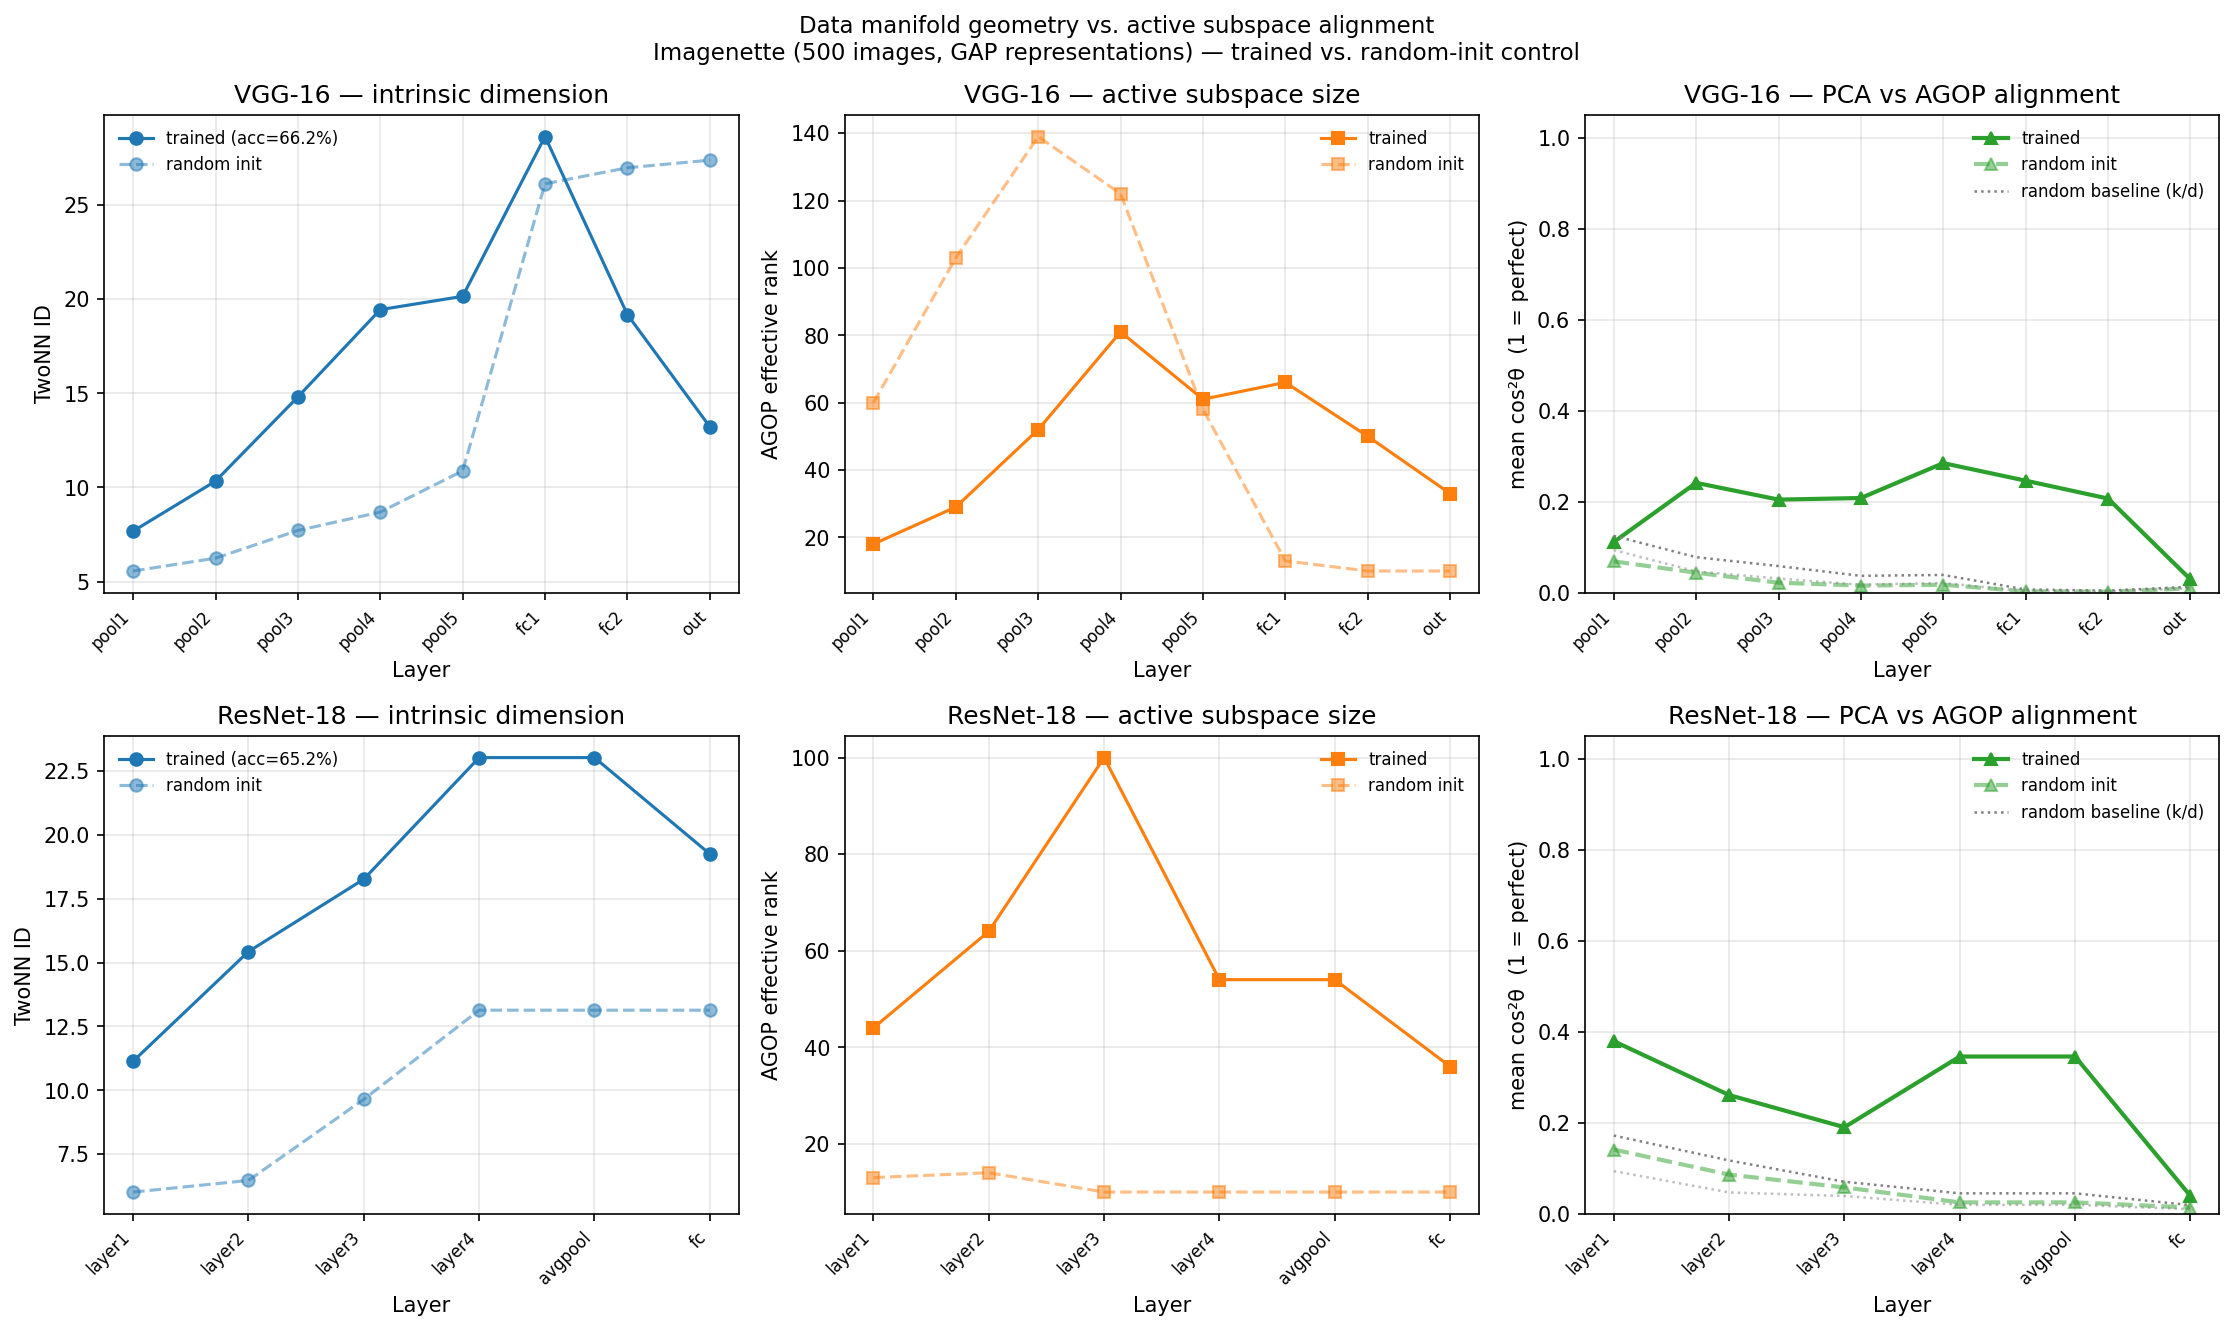
\includegraphics[width=\linewidth]{../results/alignment_experiment.png}
\caption{
\textbf{Layer-wise geometry of trained vs.\ random-init networks.}
\emph{Left}: TwoNN intrinsic dimension. \emph{Centre}: AGOP effective rank
(number of eigenvalues $>1\%$ of maximum). \emph{Right}: alignment
(mean~$\cos^2\theta$) between top-$k$ PCA and top-$k$ AGOP subspaces;
dotted line is the $k/d$ random baseline.  Solid lines: ImageNet-pretrained
weights; dashed: random initialisation.
}
\label{fig:main}
\end{figure}

\subsection{Replication: TwoNN Hunchback}

The left panels replicate the core finding of \citet{ansuini2019intrinsic}.
Trained VGG-16 rises from $\id=7.7$ at \texttt{pool1} to $28.6$ at
\texttt{fc1}, then falls to $13.2$ at the output.  Trained ResNet-18 rises
from $11.1$ at \texttt{layer1} to $23.0$ at \texttt{layer4/avgpool} and falls
to $19.2$ at \texttt{fc}.  Random-init networks show a flatter, lower profile,
consistent with \citet{ansuini2019intrinsic}'s randomised controls.

\subsection{AGOP Rank}

The centre panels show that AGOP effective rank also follows a hunchback, but
is consistently larger than the TwoNN ID.  For VGG-16, rank peaks at 81 at
\texttt{pool4} while ID peaks at 28.6 at \texttt{fc1}; for ResNet-18, rank
peaks at 100 at \texttt{layer3} while ID peaks at 23.0 later.  This
``rank overshooting'' indicates that the active subspace spans more directions
than the data manifold---the network is sensitive to perturbations in
directions that the training data does not explore.

A notable difference between architectures: random-init VGG-16 has high
AGOP rank at convolutional layers (60--139) but collapses to $\approx10$ at
FC layers.  Random-init ResNet-18 maintains low rank ($\approx10$--14) even at
early layers.  We attribute this to ResNet's skip connections, which concentrate
gradient flow through a narrow subspace even without training; VGG's
unconstrained gradient paths spread across many channels.

\subsection{Alignment}

\begin{table}[t]
\centering
\caption{Manifold-gradient alignment: mean $\cos^2\theta$ and ratio above
random baseline $k/d$.  Layers of interest highlighted.}
\label{tab:align}
\small
\begin{tabular}{llrrrr}
\toprule
Network & Layer & $d$ & ID ($k$) & $\kcos$ & ratio \\
\midrule
VGG-16 (trained) & pool1  &   64 &  7.7 & 0.111 & 0.9$\times$ \\
                  & pool5  &  512 & 20.1 & 0.285 & 7.3$\times$ \\
                  & fc1    & 4096 & 28.6 & 0.246 & 34.8$\times$ \\
                  & \textbf{fc2}    & \textbf{4096} & \textbf{19.2} & \textbf{0.207} & \textbf{44.6}$\times$ \\
                  & out    & 1000 & 13.2 & 0.029 & 2.3$\times$ \\
\midrule
VGG-16 (random)  & fc2    & 4096 & 27.0 & 0.002 & 1.0$\times$ \\
                  & out    & 1000 & 27.4 & 0.010 & 1.0$\times$ \\
\midrule
ResNet-18 (trained) & layer1   &  64 & 11.1 & 0.379 & 2.2$\times$ \\
                    & \textbf{layer4/avgpool} & \textbf{512} & \textbf{23.0} & \textbf{0.345} & \textbf{7.7}$\times$ \\
                    & fc       & 1000 & 19.2 & 0.039 & 2.1$\times$ \\
\midrule
ResNet-18 (random) & layer4/avgpool & 512 & 13.1 & 0.025 & 1.3$\times$ \\
                   & fc             & 1000 & 13.1 & 0.014 & 1.4$\times$ \\
\bottomrule
\end{tabular}
\end{table}

Table~\ref{tab:align} and the right panels of Figure~\ref{fig:main} give the
main result.  Three findings stand out.

\paragraph{(F1) Training creates alignment.}
Random-init networks sit at $\approx1\times$ the random baseline throughout.
Trained networks exceed it by $2$--$45\times$ at hidden layers.  The
structure is entirely training-induced; the architecture alone confers no
systematic alignment.

\paragraph{(F2) The last hidden layer is the alignment peak.}
VGG-16 \texttt{fc2} achieves ratio $44.6\times$, ResNet-18
\texttt{layer4}/\texttt{avgpool} achieves $7.7\times$.  These are the same
layers that \citet{ansuini2019intrinsic} identify as the generalisation
predictors via ID.  The alignment ratio and the ID together paint a coherent
picture: the final hidden representation is both maximally compressed and
maximally task-aligned.

\paragraph{(F3) The output layer destroys alignment.}
Across one linear transformation---from the last hidden layer to
logits---the ratio drops from $44.6\times$ to $2.3\times$ (VGG-16) and from
$7.7\times$ to $2.1\times$ (ResNet-18).  The logit geometry and the gradient
geometry are nearly orthogonal.  Section~\ref{sec:discussion} explains this
collapse via Neural Collapse.

% ============================================================
\section{Discussion}
\label{sec:discussion}
% ============================================================

\subsection{Connection to Neural Collapse}
\label{sec:nc}

Neural Collapse \citep{papyan2020prevalence,zhu2021geometric} establishes that
at the global minimiser of the unconstrained features model with balanced data,
classifier weight vectors and centred class means satisfy $W = \alpha M^\top$
(NC3, self-duality): the row space of $W$ equals the span of the centred class
means.  However, NC3 is a relationship between two linear objects and does
\emph{not} directly imply that the data manifold tangent space aligns with the
AGOP active subspace.  Alignment between those two objects requires within-class
variability (NC1) to have collapsed to zero---a condition that holds only
asymptotically under idealized training, not in finite-epoch practice.  No
existing theorem bridges NC3 to manifold-AGOP alignment.

\citet{beaglehole2024agop} provide a sharper mechanistic account of the
output-layer alignment drop: the AGOP drives layer-by-layer within-class
variability collapse (DNC1) across \emph{all} hidden layers via the right
singular structure of weight matrices, but the ETF class-mean geometry (DNC2)
emerges strongly \emph{only at the very last layer}.  The final linear
transformation thus constrains the active subspace to the $K$-dimensional
class-direction subspace, which is far narrower and differently oriented than
the broader data manifold directions captured at the penultimate layer.

Our finding that the last \emph{hidden} layer achieves the highest alignment,
while the \emph{output} logit layer drops sharply, is consistent with this
picture.  The output layer computes $Wh$, mapping the hidden representation
through $W$; the resulting logit-space AGOP is determined by the cross-entropy
loss curvature, which depends on the current prediction distribution rather than
the data manifold geometry, yielding generically low alignment with the data
manifold.

\subsection{Connection to Escape Dimensions}

Recent work \citep{martinelli2026escape} argues that overparameterisation
improves optimisation not by providing more ``lottery tickets''
\citep{frankle2019lottery} but by adding \emph{escape dimensions}: directions
in the loss landscape that convert sharp local minima into traversable saddle
points, making good minima more prevalent relative to bad ones.  A key
prediction is that winning subnetworks cannot be treated in isolation from the
wider network that supplied their escape-dimension context.

Our AGOP effective rank provides a complementary empirical handle.  The AGOP
is the second-order loss landscape averaged over data; its rank measures how
many dimensions the loss landscape occupies.  We find that AGOP rank is
moderate even at large layers ($d=4096$, rank $\approx50$--66 for VGG-16 FC
layers), suggesting that the effective loss-landscape dimension is much smaller
than the ambient parameter space---consistent with escape dimensions being a
real but bounded phenomenon.  The fact that AGOP rank also decreases toward
the output aligns with the intuition that, near convergence, the gradient
occupies fewer and fewer directions as the loss flattens.

\subsection{What the Alignment Measures---and What It Doesn't}

The alignment ratio tells us how much of the data manifold's intrinsic
geometry is ``seen'' by the gradient, and vice versa.  A ratio of $45\times$
means that knowing which directions the data varies in is highly informative
about which directions the loss varies in---a much stronger relationship than
random.  But a ratio of $45\times$ with $\kcos=0.21$ is still far from
perfect alignment ($\kcos=1$).  This residual misalignment could reflect:
(a) the approximation of the data manifold tangent space by global PCA;
(b) the spatial-mean approximation for conv layer AGOP;
(c) genuine misalignment between unused data directions and actively-used
gradient directions.

Disentangling these contributions requires finer tools---local tangent space
estimation, exact AGOP computation for spatial layers, and larger-scale
experiments across more architectures---which we leave to future work.

\subsection{Limitations}

\begin{itemize}
\item \textbf{Small scale.}  We study two architectures and $N=500$ images.
  The alignment scores may shift with more data, especially for early layers
  where $N$ is a binding constraint on TwoNN accuracy.

\item \textbf{Imagenette vs.\ ImageNet.}  Models are trained on ImageNet
  (1000 classes) but evaluated on Imagenette (10 classes).  The AGOP is
  computed on Imagenette images with their correct ImageNet class indices,
  so the gradient is class-specific; but the data manifold reflects only 10
  of the 1000 classes.

\item \textbf{GAP approximation.}  For convolutional layers, we apply global
  average pooling to both activations and gradients.  This discards spatial
  structure and may understate alignment for layers where spatial information
  is functionally important.

\item \textbf{Single time point.}  We measure alignment in a trained network.
  Training dynamics of alignment---whether it builds monotonically or
  non-monotonically, and whether faster alignment predicts faster
  generalisation---are unexplored.
\end{itemize}

% ============================================================
\section{Conclusion}
\label{sec:conclusion}
% ============================================================

We have shown that trained CNN representations are not merely compressed (low
intrinsic dimension) but \emph{task-aligned}: the directions that span the
data manifold are the same directions along which the loss varies.  This
alignment is strongest at the last hidden layer---the known generalisation
predictor---reaches $35$--$45\times$ above chance for VGG-16 FC layers, and
collapses to $\approx2\times$ at the output layer.  Random-init networks show
no such alignment.

These findings suggest that the intrinsic dimension story of
\citet{ansuini2019intrinsic} is incomplete: what matters is not just how
much the representation is compressed, but whether it is compressed along the
dimensions that drive the task.  The drop at the output layer, explicable via
Neural Collapse geometry, shows that task alignment is a property of the
penultimate representation rather than the final classification surface.

Future directions include: extending to more architectures and more images;
tracking alignment during training; probing whether higher alignment at
intermediate layers is causally linked to better generalisation (e.g.\ via
targeted interventions that decorrelate the subspaces); and connecting the
alignment trajectory to the escape-dimensions account of why overparameterised
networks train so readily.

% ============================================================
\section*{Reproducibility Statement}

All code, the trained model checkpoints (loaded from torchvision), and the
Imagenette dataset are publicly available.  The complete experiment script and
TwoNN implementation are at
\url{https://github.com/kilojoules/manifold-active-subspace}.
The dataset downloads automatically on first run ($\approx100$~MB).
Experiments complete in under one hour on a laptop CPU or Apple MPS device.

\section*{Author Contributions}

Single-author work.

% ============================================================
\bibliography{references}
\bibliographystyle{abbrvnat}

\end{document}
